\documentclass[10.5pt,a4paper]{article}
\usepackage[utf8]{inputenc}
\usepackage[T1]{fontenc}
\pdfmapfile{+lm.map}
\pdfmapfile{+cm.map}
\pdfmapfile{+symbols.map}
\IfFileExists{french.ldf}{\usepackage[french]{babel}}{\usepackage[provide=*,french]{babel}}
\IfFileExists{lmodern.sty}{\usepackage{lmodern}}{}
\usepackage{amsmath,amssymb}
\usepackage{graphicx}
\usepackage{array,tabularx,float}
\PassOptionsToPackage{hyphens}{url}
\usepackage[dvipsnames]{xcolor}
\usepackage{tocloft}
\usepackage[colorlinks=true,linkcolor=MidnightBlue,citecolor=MidnightBlue,urlcolor=RoyalBlue,linktoc=all]{hyperref}
\definecolor{bleuSombre}{HTML}{153C61}
\definecolor{bleuRoyal}{HTML}{1768A4}
\definecolor{bleuClair}{HTML}{45A8CA}
\renewcommand{\contentsname}{Table des matières}
\renewcommand{\cfttoctitlefont}{\color{bleuSombre}\LARGE\bfseries}
\renewcommand{\cftaftertoctitle}{\par\vspace{0.5em}{\color{bleuClair}\rule{\textwidth}{1.15pt}}\vspace{1.0em}}
\renewcommand{\cftsecfont}{\color{bleuSombre}\bfseries}
\renewcommand{\cftsecpagefont}{\color{bleuSombre}\bfseries}
\renewcommand{\cftsubsecfont}{\color{bleuRoyal}}
\renewcommand{\cftsubsecpagefont}{\color{bleuRoyal}}
\renewcommand{\cftdotsep}{1.7}
\setlength{\cftbeforesecskip}{0.48em}
\setlength{\cftbeforesubsecskip}{0.12em}
\setcounter{tocdepth}{2}
\usepackage[a4paper,margin=2.1cm]{geometry}
% Keep the original lightweight typography; permit proper line breaks in long references.
\IfFileExists{url.sty}{\usepackage{url}}{\newcommand{\url}[1]{{\small\ttfamily #1}}}
\sloppy

\setlength{\parskip}{3pt}
\renewcommand{\arraystretch}{1.15}
\newcommand{\code}[1]{\texttt{#1}}
\newcommand{\pkg}{\code{ldaR6}}
\newcommand{\bm}[1]{\mathbf{#1}}
\newcommand{\T}{^{\top}}

\title{
\includegraphics[width=4.2cm]{figures/logo_lyon2.jpg}\\[8pt]
\textbf{Analyse discriminante lin\'eaire pr\'edictive : un package R6 et une application Shiny}\\[2pt]
\large Package \pkg\ --- M2 SISE, Programmation R, 2026--2027}
\author{MAMPOUYA CLARK Chancy Loïc Franlly\\[3pt]\small Travail individuel}
\date{Rendu du 15 novembre 2026}

\begin{document}
% Pagination pr\'eliminaire en chiffres romains : garde i, r\'esum\'e ii, sommaire iii.
\pagenumbering{roman}
\maketitle
\clearpage

% R\'esum\'e sur une page d\'edi\'ee, avec des marges g\'en\'ereuses.
\phantomsection
\addcontentsline{toc}{section}{R\'esum\'e}
\noindent{\color{bleuRoyal}\small\bfseries M2 SISE \quad/\quad PROGRAMMATION R \quad/\quad 2026--2027}\par
\vspace{1.3em}
{\color{bleuSombre}\LARGE\bfseries R\'esum\'e}\par
\vspace{0.55em}\noindent{\color{bleuClair}\rule{\textwidth}{1.15pt}}\par
\vspace{1em}
\noindent\begin{minipage}{\textwidth}\normalsize\setlength{\parindent}{0pt}
Je pr\'esente \pkg, un package R d'analyse discriminante lin\'eaire (ADL) pr\'edictive dont le c\oe ur est impl\'ement\'e \emph{from scratch} avec une classe R6. Il propose les m\'ethodes \code{fit}, \code{predict} et \code{predict\_proba}, les fonctions de classement, le lambda de Wilks, des tests de pertinence et la s\'election pas-\`a-pas des variables. Les variables cat\'egorielles sont recod\'ees et les calculs optimis\'es pour de grands volumes. Une application Shiny permet de charger les donn\'ees, visualiser les r\'esultats et pr\'edire une classe individuellement ou par fichier. Une documentation en anglais, des tests unitaires et des benchmarks comparatifs avec \code{MASS::lda} compl\`etent le projet.
\end{minipage}
\vfill
\noindent{\color{bleuClair}\rule{\textwidth}{0.55pt}}\\[4pt]
{\color{bleuSombre}\small Rapport individuel \hfill Package \pkg}
\clearpage

% Sommaire bleu : num\'erotation romaine conserv\'ee.
\noindent{\color{bleuRoyal}\small\bfseries M2 SISE \quad/\quad PROGRAMMATION R \quad/\quad 2026--2027}\par
\vspace{1.0em}
\tableofcontents
\vfill
\noindent{\color{bleuClair}\rule{\textwidth}{0.55pt}}\\[4pt]
{\color{bleuSombre}\small Rapport individuel \hfill Package \pkg}
\clearpage

% Retour aux chiffres arabes pour le corps du rapport, \`a partir de 1.
\pagenumbering{arabic}

%=====================================================================
\section{Cahier des charges et d\'emarche}
Le sujet officiel \cite{sujet} demande un package R install\'able depuis GitHub, dont le c\oe ur de l'ADL est programm\'e par l'auteur selon la norme R6, avec : un constructeur, \code{\$fit(X, y)}, \code{\$predict(X)}, \code{\$predict\_proba(X)}, \code{\$print()}, \code{\$summary()} et des propri\'et\'es expos\'ees ; les coefficients du mod\`ele et des indicateurs d'\'evaluation globale et de pertinence des variables ; une strat\'egie pour les explicatives cat\'egorielles et une pour la s\'election de variables ; une application Shiny (chargement, choix des variables explicatives et illustratives, calculs, pr\'ediction individuelle et par fichier) ; un rapport \LaTeX\ ($\leq 12$ pages), une aide et un tutoriel en anglais, une archive de secours. La rapidit\'e et la prise en compte des grandes volum\'etries sont des crit\`eres d'\'evaluation. Le lambda de Wilks et les tests associ\'es correspondent \`a des choix d'impl\'ementation pour l'interpr\'etation statistique. L'ouvrage de r\'ef\'erence de Ricco Rakotomalala \cite{rako} guide la pr\'esentation statistique.

Ma d\'emarche a \'et\'e : (i) formuler l'algorithme \`a partir de \emph{statistiques suffisantes} (moyennes par classe et matrices de sommes de carr\'es et de produits crois\'es, SSCP) ; (ii) faire reposer tous les tests et la s\'election sur ces seules matrices $p\times p$, de sorte que leur co\^ut ne d\'epende plus de $n$ ; (iii) valider chaque brique contre des r\'ef\'erences ind\'ependantes (\code{MASS::lda}, \code{stats::manova}, identit\'es math\'ematiques de l'ADL) ; (iv) mesurer les performances et chasser les d\'efaillances.

%=====================================================================
\section{Fondements th\'eoriques}\label{sec:theorie}
\subsection{Mod\`ele et r\`egle de d\'ecision}
Soit $n$ individus d\'ecrits par $p$ variables num\'eriques $\bm{x}\in\mathbb{R}^p$ et r\'epartis en $K$ classes d'effectifs $n_k$. On note $\bm{m}_k$ le centre de la classe $k$, $\bm{m}$ le centre global et
\begin{equation}
\bm W=\sum_{k=1}^K\sum_{i\in k}(\bm x_i-\bm m_k)(\bm x_i-\bm m_k)\T,\quad
\bm B=\sum_{k=1}^K n_k(\bm m_k-\bm m)(\bm m_k-\bm m)\T,\quad \bm T=\bm W+\bm B .
\end{equation}
Sous l'hypoth\`ese gaussienne \`a covariance commune $\bm\Sigma$ estim\'ee par $\hat{\bm\Sigma}=\bm W/(n-K)$, la r\`egle de Bayes est lin\'eaire : la \emph{fonction de classement} de la classe $k$ est
\begin{equation}
f_k(\bm x)=\ln\pi_k-\tfrac12\bm m_k\T\hat{\bm\Sigma}^{-1}\bm m_k+(\hat{\bm\Sigma}^{-1}\bm m_k)\T\bm x ,
\label{eq:fk}
\end{equation}
avec $\pi_k$ la probabilit\'e a priori (proportionnelle aux effectifs, \'egale, ou fournie). L'individu est affect\'e \`a $\arg\max_k f_k$ et les probabilit\'es a posteriori sont $P(k|\bm x)=e^{f_k}/\sum_j e^{f_j}$ (calcul\'ees apr\`es soustraction du maximum pour la stabilit\'e num\'erique). Les coefficients du score de classement sont les composantes de $\hat{\bm\Sigma}^{-1}\bm m_k$ ; la constante int\`egre la probabilit\'e a priori par le terme $\ln\pi_k$.

\subsection{Axes discriminants}
Les axes canoniques r\'esolvent $\bm B\bm a=\ell\,\hat{\bm\Sigma}\bm a$. Comme $\bm B=\bm D\bm D\T$ avec $\bm D=[\sqrt{n_k}(\bm m_k-\bm m)]_k$ de rang $\le K-1$, le probl\`eme se ram\`ene \`a la matrice $K\times K$ $\bm C=\bm D\T\hat{\bm\Sigma}^{-1}\bm D$ : si $\bm C\bm v=\ell\bm v$, alors $\bm a=\hat{\bm\Sigma}^{-1}\bm D\bm v/\sqrt{\ell}$ v\'erifie $\bm a\T\hat{\bm\Sigma}\bm a=1$. On \'evite ainsi toute d\'ecomposition propre $p\times p$ (voir \S\ref{sec:perf}). Les valeurs propres $\lambda_j=\ell_j/(n-K)$ de $\bm W^{-1}\bm B$ donnent les corr\'elations canoniques $\sqrt{\lambda_j/(1+\lambda_j)}$.

\subsection{Lambda de Wilks et tests}
Le lambda de Wilks mesure le pouvoir discriminant global :
\begin{equation}
\Lambda=\frac{|\bm W|}{|\bm T|}=\prod_{j}\frac1{1+\lambda_j}\in[0,1]\quad(\text{petit}=\text{bon}).
\end{equation}
Pour $q$ variables, $h=K-1$ degr\'es de libert\'e d'hypoth\`ese et $e$ d'erreur, l'approximation de Rao donne $F=\frac{1-\Lambda^{1/t}}{\Lambda^{1/t}}\cdot\frac{df_2}{df_1}$ avec $df_1=qh$, $df_2=wt-\frac{qh-2}2$, $w=e+h-\frac{q+h+1}{2}$ et $t=\sqrt{\frac{q^2h^2-4}{q^2+h^2-5}}$ ($t=1$ si le d\'enominateur est $\le0$) ; elle est exacte pour $q=1$ ou $h\le2$. Le package fournit aussi les traces de Pillai et de Hotelling--Lawley, la plus grande racine de Roy et le $\chi^2$ de Bartlett (global puis par axe).

\paragraph{Test partiel.} L'apport d'une variable (ou d'un bloc $B$ de colonnes) $j$ \emph{sachant} les autres est $\Lambda(j|S)=\Lambda(S\cup j)/\Lambda(S)$ ; il se lit directement sur les inverses des SSCP du mod\`ele courant :
\begin{equation}
\Lambda(B\,|\,S\setminus B)=\frac{|(\bm T_{SS}^{-1})_{BB}|}{|(\bm W_{SS}^{-1})_{BB}|},
\end{equation}
test\'e par la loi de Rao avec $q=|B|$ et $e=n-K-(|S|-q)$. Pour les candidats \`a l'entr\'ee, on utilise les SSCP r\'esiduelles apr\`es r\'egression sur $S$, calcul\'ees pour tous les candidats d'un coup (op\'erations matricielles, \S\ref{sec:select}). Enfin, les distances de Mahalanobis $D^2_{kl}=(\bm m_k-\bm m_l)\T\hat{\bm\Sigma}^{-1}(\bm m_k-\bm m_l)$ sont test\'ees par $F=\frac{(n-K-p+1)\,n_kn_l}{p(n-K)(n_k+n_l)}D^2_{kl}$.

%=====================================================================
\section{Architecture du programme}\label{sec:archi}
\subsection{Modules R}
\begin{center}
\begin{tabularx}{\textwidth}{|l|X|}\hline
\textbf{Fichier} & \textbf{R\^ole}\\\hline
\code{R/LDA.R} & classe R6 \code{LDA} : \code{fit}, \code{predict}, \code{predict\_proba}, \code{decision\_function}, \code{transform}, \code{score}, \code{confusion}, \code{cross\_validate}, \code{variable\_audit}, \code{project\_illustrative}, \code{print}, \code{summary}, \code{plot} ; propri\'et\'es en lecture seule (liaisons actives)\\\hline
\code{R/encoding.R} & apprentissage (\code{.make\_encoder}) et application (\code{.apply\_encoder}) du codage des cat\'egorielles\\\hline
\code{R/stats\_utils.R} & log-d\'eterminant, inverses (Cholesky, pseudo-inverse), F de Rao, statistiques partielles d'entr\'ee et de sortie\\\hline
\code{R/selection.R} & s\'election pas-\`a-pas (forward, backward, both) sur les SSCP\\\hline
\code{R/utils\_public.R} & \code{read\_data}, \code{simulate\_lda\_data}, \code{run\_app}, m\'ethodes S3 (\code{predict}, \code{coef}, \code{summary}, \code{plot})\\\hline
\code{inst/shiny/app/app.R} & application Shiny\\\hline
\end{tabularx}
\end{center}
Les fonctions internes sont pures (SSCP en entr\'ee, statistiques en sortie), donc testables sans donn\'ees brutes ; la classe orchestre.

\subsection{Interface de la classe}
\code{LDA\$new(priors, encoding, selection, alpha\_enter, alpha\_stay, max\_vars, shrinkage, na\_action, chunk\_size)} ne fait que stocker les param\`etres. \code{\$fit(X, y)} renvoie l'objet (cha\^inage) et remplit un enregistrement priv\'e expos\'e par des liaisons actives. Les principaux objets g\'en\'er\'es sont :
\begin{center}
\begin{tabularx}{\textwidth}{|l|X|}\hline
\code{\$coefficients} & matrice $(p+1)\times K$ des fonctions de classement (constante en premi\`ere ligne)\\\hline
\code{\$wilks} & \code{global} (lambda, $F$, $df_1$, $df_2$, $p$), \code{multivariate} (Wilks, Pillai, Hotelling--Lawley, Roy), Bartlett\\\hline
\code{\$variables} & par variable : lambda univari\'e et partiel, $F$, $p$, \code{status} $\in\{$contributing, redundant, uninformative$\}$\\\hline
\code{\$canonical} & coefficients des axes, valeurs propres, corr\'elations canoniques et tests par axe, structure, centro\"ides\\\hline
\code{\$distances} & $D^2$ entre classes et $p$-values\\\hline
\code{\$selected}, \code{\$selection\_history} & variables retenues ; chemin (\'etape, action, lambda partiel, $F$, $p$, Wilks cumul\'e)\\\hline
\code{\$confusion\_train}, \code{\$accuracy\_train}, \code{\$scores\_train} & r\'esultats en resubstitution et coordonn\'ees factorielles\\\hline
\code{\$means}, \code{\$pooled\_cov}, \code{\$priors}, \code{\$classes}, \code{\$features} & ingr\'edients du mod\`ele et description des variables\\\hline
\end{tabularx}
\end{center}
Les g\'en\'eriques R usuels sont aussi disponibles (\code{predict(m, newdata, type="prob")}, \code{coef}, \code{summary}, \code{plot}).

\subsection{Choix d'architecture : tout int\'egr\'e plut\^ot qu'un pipeline}
Le sujet autorise soit l'int\'egration des traitements (cat\'egorielles, s\'election) dans le mod\`ele, soit un pipeline s\'epar\'e fa\c{c}on scikit-learn. J'ai choisi l'\textbf{int\'egration} dans la classe, avec des modules internes distincts, pour quatre raisons :
\begin{enumerate}
\item \emph{Pas de fuite d'information} : l'encodeur (niveaux, colonnes) et la s\'election sont appris sur l'\'echantillon d'apprentissage puis rejou\'es \`a l'identique par \code{predict}. La validation crois\'ee refait tout le pipeline dans chaque pli (\code{cross\_validate}), ce qui \'evite l'optimisme classique d'une s\'election faite sur toutes les donn\'ees.
\item \emph{Performance} : la s\'election r\'eutilise les SSCP $\bm W$ et $\bm T$ d\'ej\`a calcul\'ees pour le mod\`ele ; un pipeline s\'epar\'e les recalculerait ou imposerait de les faire circuler.
\item \emph{Pr\'ediction minimale} : apr\`es s\'election, l'encodeur est restreint aux colonnes utiles, donc \code{predict} n'exige que les variables retenues (utile pour le formulaire individuel de Shiny).
\item \emph{Utilisabilit\'e} : un seul objet, un seul contrat \code{fit/predict}.
\end{enumerate}
Contrepartie assum\'ee : le crit\`ere de s\'election (Wilks) est li\'e \`a l'ADL et ne se d\'ecouple pas ; la maintenance exige de respecter la fronti\`ere entre fonctions pures et classe, appliqu\'ee fichier par fichier.

%=====================================================================
\section{Choix m\'ethodologiques}
\subsection{Variables explicatives cat\'egorielles}\label{sec:cat}
Le calcul matriciel de l'ADL exige des colonnes num\'eriques. Le codage est effectu\'e \emph{en amont}, sans toucher \`a l'algorithme, avec trois options (param\`etre \code{encoding}) :
\begin{itemize}
\item \textbf{dummy} (d\'efaut) : $k-1$ indicatrices, la premi\`ere modalit\'e servant de r\'ef\'erence. C'est le choix qui conserve $\hat{\bm\Sigma}$ inversible ; chaque coefficient s'interpr\`ete par rapport \`a la modalit\'e de r\'ef\'erence.
\item \textbf{one-hot} : $k$ indicatrices. Leur somme vaut 1 pour tout individu, donc $\hat{\bm\Sigma}$ est singuli\`ere (colinéarit\'e parfaite). Le package bascule alors sur une pseudo-inverse de Moore--Penrose et \'emet un avertissement. Un test unitaire a v\'erifi\'e que les pr\'edictions sont strictement identiques \`a celles du codage dummy : les deux param\'etrisations engendrent le m\^eme espace, seul l'aspect des coefficients change.
\item \textbf{label} : un entier par variable. Compact mais il impose un ordre et des distances entre modalit\'es : acceptable seulement pour des facteurs ordonn\'es, trompeur sinon.
\end{itemize}
\textbf{Cons\'equences.} Des indicatrices ne sont pas gaussiennes : l'ADL reste un classifieur lin\'eaire raisonnable (pratique courante) mais les tests de Wilks deviennent approximatifs pour les facteurs tr\`es d\'es\'equilibr\'es. Une modalit\'e pr\'esente dans une seule classe sans variance interne produit une colonne d\'eg\'en\'er\'ee, retir\'ee avec avertissement. Lors de la s\'election, une cat\'egorielle entre ou sort \emph{comme bloc}, test\'ee par un lambda partiel multivari\'e ($q=k-1$) : on \'evite de garder une modalit\'e isol\'ee. Une alternative que je n'ai pas impl\'ement\'ee est DISQUAL (ACM puis ADL, \cite{saporta}).

\subsection{S\'election de variables et analyse des contributions}\label{sec:select}
Crit\`ere : le lambda de Wilks partiel et son test F de Rao (seuils \code{alpha\_enter}, \code{alpha\_stay}, d\'efaut $0{,}05$). Trois strat\'egies : \emph{forward}, \emph{backward} et \emph{both} (pas-\`a-pas).

\begin{small}
\begin{verbatim}
SELECT(W, T, blocs, direction, a_in, a_out):
  S <- {} (forward/both)  ou  tous les blocs (backward)
  repeter (garde-fou : 4*nb_blocs + 5 tours)
    si direction in {backward, both}:                # sortie
        pour chaque bloc B de S : p_B <- test(Lambda(B | S\B))   # via inverses de W_SS, T_SS
        si max p_B > a_out : retirer ce bloc ; (continuer si backward)
    si direction in {forward, both} et |S| < max_vars:  # entree
        pour tous les candidats c hors de S : Lambda(c | S) <- det(W_res)/det(T_res)
           avec W_res = W_cc - W_cS W_SS^-1 W_Sc   (vectorise pour les blocs de taille 1)
        c* <- candidat de plus petite p-value ; si p <= a_in : ajouter c*
  jusqu'a stabilite ;  retourner S et l'historique (etape, action, Lambda, F, p, Wilks)
\end{verbatim}
\end{small}

Chaque \'etape co\^ute $O(|S|^2p)$ pour tous les candidats simultan\'ement, ind\'ependamment de $n$. Pour \emph{toutes} les variables, y compris les non retenues, \code{\$variables} donne le test univari\'e (variable seule) et le test partiel (sachant le mod\`ele final). Le package en d\'eduit le \code{status} demand\'e par le sujet :
\emph{contributing} (apporte de l'information sachant les autres), \emph{redundant} (informative seule mais sans apport additionnel : par exemple \code{income\_copy}, copie bruit\'ee de \code{income}) et \emph{uninformative} (aucun lien avec la cible). Les variables \emph{perturbatrices} sont d\'etect\'ees par \code{variable\_audit} : une variable est perturbatrice si son retrait \emph{augmente} la pr\'ecision en validation crois\'ee (m\^emes plis, m\^eme graine). La Figure~\ref{fig:imp} montre le r\'esultat sur les donn\'ees d\'emo : les cinq variables num\'eriques utiles, \code{housing} et \code{education} sont retenues ; \code{income\_copy} (redondante), \code{noise1}, \code{noise2} et \code{job} sont \'ecart\'ees. \textbf{Limite} : les $p$-values apr\`es s\'election sont optimistes ; seule la validation crois\'ee incluant la s\'election donne une pr\'ecision honn\^ete.

\begin{figure}[H]\centering
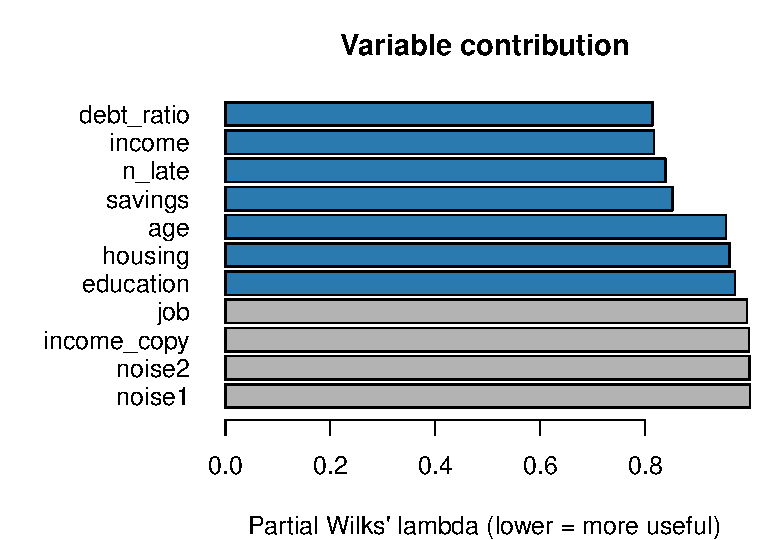
\includegraphics[width=0.62\textwidth]{figures/fig_importance.pdf}
\caption{Lambda de Wilks partiel par variable (\code{credit\_demo}, s\'election pas-\`a-pas) ; en bleu les variables apportant de l'information sachant les autres.}\label{fig:imp}
\end{figure}

\subsection{Singularit\'e, grande dimension et valeurs manquantes}
Lorsque $\hat{\bm\Sigma}$ est singuli\`ere ($p\ge n-K$, colinéarit\'e), l'inversion de Cholesky est remplac\'ee par une pseudo-inverse spectrale avec avertissement explicite. L'option \code{shrinkage}$=\gamma$ remplace $\hat{\bm\Sigma}$ par $(1-\gamma)\hat{\bm\Sigma}+\gamma\,\mathrm{diag}(\hat{\bm\Sigma})$ (r\'etr\'ecissement vers la diagonale, \cite{friedman,schafer}) : toujours inversible, \emph{invariant d'\'echelle}. La premi\`ere version r\'etr\'ecissait vers $\bar s\,\bm I$ ; un test a montr\'e qu'une variable de grande variance (\code{savings}) dominait alors le terme et d\'et\'eriorait la pr\'ecision (69\,\% au lieu de 82\,\%)  ; ce choix a \'et\'e corrig\'e. Les tests partiels sont d\'esactiv\'es (\code{NA}) si $\bm W_{SS}$ est singuli\`ere, car ils n'ont alors pas de sens. Les lignes incompl\`etes sont retir\'ees avec avertissement (ou erreur selon \code{na\_action}) ; en pr\'ediction, une ligne incompl\`ete ou \`a modalit\'e inconnue re\c{c}oit \code{NA}.

%=====================================================================
\section{Impl\'ementation et performances}\label{sec:perf}
\subsection{Algorithme de \code{fit}}
\begin{small}
\begin{verbatim}
FIT(X, y):
  1 valider ; retirer NA ; apprendre encodeur ; M <- encoder(X)     # O(np)
  2 moyennes <- rowsum(M, y) ; B <- crossprod(sqrt(n_k)*(m_k-m))
  3 W <- 0 ; pour chaque bloc de chunk_size lignes :
      W += crossprod(M_bloc - m[y_bloc])                             # O(np^2)
  4 retirer colonnes sans variance intra ; T <- W + B
  5 si selection != none : S <- SELECT(W, T, ...)
  6 Sigma <- W_SS/(n-K) ; Sigma <- (1-g)*Sigma + g*diag(Sigma)
      Sinv <- chol2inv(chol(Sigma))  # repli pseudo-inverse si necessaire
  7 coef <- Sinv t(m_S) ; const <- ln(prior) - 0.5 colSums(t(m_S)*coef)
  8 Wilks <- exp(logdet W_SS - logdet T_SS) ; Rao F ; Bartlett ; D^2
      axes via C = D' Sinv D (K x K)
  9 Z <- M_S coef + const ; confusion ; tableau des tests par variable
\end{verbatim}
\end{small}
Complexit\'e : $O(np^2+p^3+Kp^2)$, avec $np^2$ dominant pour les donn\'ees longues. Les points d'optimisation sont : \code{crossprod} (BLAS) ; \code{rowsum} (C) pour les centres ; accumulation par blocs de lignes (temporaires limit\'es, r\'esultat identique, test unitaire \`a \code{chunk\_size=700}) ; axes canoniques par une matrice $K\times K$ plut\^ot qu'une d\'ecomposition $p\times p$ ; log-d\'eterminants par Cholesky (pas de d\'epassement) ; tests partiels vectoris\'es. La pr\'ediction est une multiplication matricielle $O(npK)$.

\subsection{Banc d'essai}
Les chiffres comparatifs du tableau et de la figure ci-dessous proviennent du banc d'essai initial (fichier \code{benchmarks/benchmark\_results.csv}) ; ils n'ont pas \'et\'e reproduits sur la version corrig\'ee. Ils sont conserv\'es comme \emph{r\'esultats historiques} et ne doivent pas \^etre confondus avec les nouvelles mesures locales. Le script \code{benchmarks/benchmark.R} compare \code{LDA\$fit} \`a \code{MASS::lda} sur donn\'ees gaussiennes simul\'ees (\code{simulate\_lda\_data}), temps m\'edian de 1 \`a 3 r\'ep\'etitions. Pour chaque cas, les classes pr\'edites co\"incident dans 100\,\% des cas avec celles de \code{MASS::lda} (contr\^ole sur les 5\,000 premi\`eres lignes).
\begin{center}
\begin{tabular}{|l|r|r|r|r|r|}\hline
Cas & $n$ & $p$ & \code{MASS::lda} (s) & \pkg\ (s) & gain\\\hline
long & $10^5$ & 10 & 0,17 & 0,12 & $1{,}4\times$\\
long & $10^6$ & 10 & 2,79 & 1,57 & $1{,}8\times$\\
long & $10^6$ & 50 & 31,03 & 9,04 & $3{,}4\times$\\
interm\'ediaire & 5\,000 & 50 & 0,14 & 0,13 & $1{,}1\times$\\
interm\'ediaire & 20\,000 & 200 & 5,95 & 1,40 & $4{,}3\times$\\\hline
\end{tabular}
\end{center}
\begin{figure}[H]\centering
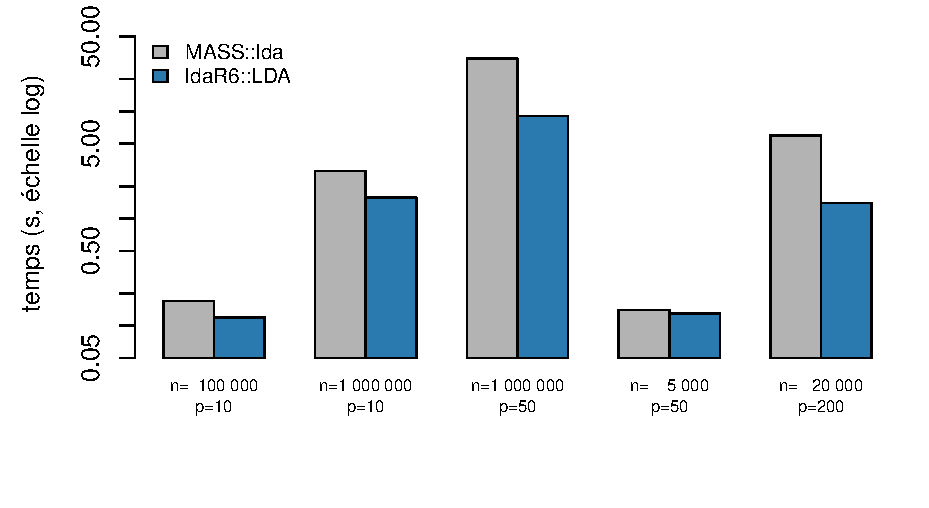
\includegraphics[width=0.7\textwidth]{figures/fig_bench.pdf}
\caption{Temps d'ajustement (\'echelle logarithmique), donn\'ees longues et interm\'ediaires.}
\end{figure}
\textbf{Donn\'ees larges} ($n=200$, $K=3$ ; \code{MASS::lda} non compar\'e car $p>n-K$ rend la covariance singuli\`ere) :
\begin{center}
\begin{tabular}{|l|r|r|r|}\hline
$p$ & pseudo-inverse (s) & \code{shrinkage=0.2} (s) & \code{selection="forward"} (s)\\\hline
500 & 0,58 & 0,33 & 0,30\\
2\,000 & 14,14 & 4,77 & 1,17\\\hline
\end{tabular}
\end{center}
La pseudo-inverse co\^ute une d\'ecomposition propre $O(p^3)$ ; le r\'etr\'ecissement la remplace par Cholesky (3$\times$ plus rapide \`a $p=2000$) et la s\'election pas-\`a-pas, qui n'inverse que de petites matrices, est la plus rapide. Un autre essai a rev\'el\'e un gain de $\times 13$ apr\`es avoir supprim\'e deux d\'ecompositions propres $p\times p$ (22\,s $\to$ 1,7\,s pour $p=1000$). Pour $p\gg n$, la pr\'ecision d'apprentissage d'une pseudo-inverse n'a pas de valeur pr\'edictive ($0{,}555$ pour $p=2\,000$ alors que seules 5 variables informent) : on utilise \code{cross\_validate} pour juger, la s\'election ou le r\'etr\'ecissement pour fiabiliser. Validation crois\'ee 10 plis ($n=2\cdot10^4$, $p=50$) : 1,5\,s ; s\'election pas-\`a-pas : 0,9\,s.


\paragraph{Mesures locales compl\'ementaires (novembre 2026).}
Sur la version test\'ee sous R 4.4.2 (Windows), trois appels distincts \`a une fonction de mesure bas\'ee sur \code{system.time} ont fourni les temps \emph{elapsed} suivants :
\begin{center}
\begin{tabular}{|r|r|r|r|r|}\hline
$n$ (apprentissage) & $p$ & $n_{\rm pred}$ & fit (s) & predict (s)\\\hline
10\,000 & 10 & 1\,000 & 0,06 & 0,00\\
100\,000 & 10 & 10\,000 & 0,45 & 0,01\\
100\,000 & 10 & 100\,000 & 0,28 & 0,05\\\hline
\end{tabular}
\end{center}
Ces temps sont ponctuels, arrondis \`a 0,01\,s ; \code{0,00} n'est pas un temps nul. Ils ne mesurent ni la m\'emoire maximale ni un gain face \`a \code{MASS::lda} sur cette machine. Une comparaison reproductible n\'ecessite plusieurs r\'ep\'etitions et la m\^eme configuration de donn\'ees.

\paragraph{M\'emoire et reproductibilit\'e.} Le traitement par blocs ne supprime pas la matrice encod\'ee compl\`ete : la m\'emoire est de l'ordre de $O(np+p^2)$, avec plusieurs matrices $p\times p$. Une seule matrice dense de $10\,000\times10\,000$ doubles occupe environ 800 Mo. Les temps d'apprentissage et de pr\'ediction doivent \^etre mesur\'es s\'epar\'ement ; le script conserve d\'esormais les versions et les informations mat\'erielles disponibles. La taille de l'objet R ne mesure pas le pic m\'emoire du processus.

\subsection{Robustesse}
Le banc d'essai a servi de test de charge : \`a $n=10^6$ il a r\'ev\'el\'e un d\'epassement d'entier dans le test de distance ($n_kn_l$ calcul\'e en entiers), corrig\'e en stockant les effectifs en r\'eels. Les cas limites suivants sont couverts par des tests : colonne constante (retir\'ee, avertissement), facteur \`a un niveau, classe \`a une seule observation, deux classes, $p>n$, NA en apprentissage et en pr\'ediction, modalit\'e inconnue, colonne manquante (erreur explicite), objet non ajust\'e (erreur explicite), invariance \`a l'\'echelle et au d\'ecalage d'une variable.

%=====================================================================
\section{Validation des calculs}
\paragraph{R\'ef\'erences et tests fournis.} Les comparaisons num\'eriques de pr\'ecision qui suivent proviennent de la suite initiale ; une ex\'ecution s\'epar\'ee de tous les tests \code{testthat} reste \`a documenter pour la version corrig\'ee. Sur \code{iris} : probabilit\'es a posteriori identiques \`a \code{MASS::lda} \`a $5\cdot10^{-15}$ pr\`es, coefficients des axes \`a $10^{-14}$ ; lambda de Wilks, $F$ de Rao et trace de Pillai identiques \`a \code{stats::manova} ($\Lambda=0{,}02344$, $F(8,288)=199{,}1$) ; lambda partiel confront\'e \`a sa d\'efinition (mod\`ele complet / r\'eduit) ; fonctions de classement recalcul\'ees ligne \`a ligne \`a partir de l'\'equation~(\ref{eq:fk}). Les coefficients de \code{Sepal.Length} (23,54417 ; 15,69821 ; 12,44585) sont reproduits dans l'exemple num\'erique de l'annexe~A.

\paragraph{Port\'ee de la validation.} Les comparaisons num\'eriques portent sur les fonctions impl\'ement\'ees en R et les r\'ef\'erences \code{MASS::lda} et \code{stats::manova}. Les r\'esultats de la suite initiale sont distingu\'es des mesures locales r\'ecentes.


\paragraph{Exemple de r\'esultats.} Le test initial de \code{credit\_demo} ($n=900$, 3 classes) avec 11 variables candidates s\'electionne 7 variables (dont \code{education}) : $\Lambda=0{,}232$, pr\'ecision 82,6\,\% en resubstitution et 81,6\,\% en validation crois\'ee 10 plis. Dans la d\'emonstration locale r\'ecente, avec seulement 7 variables candidates (sans \code{education}), la configuration sans s\'election atteint 81,6\,\% (entra\^inement et validation crois\'ee 5 plis) ; la s\'election \code{both} retire \code{job}, conserve 6/7 variables et obtient 81,8\,\% \`a l'entra\^inement, 81,0\,\% en validation crois\'ee 5 plis ($\Lambda=0{,}239$). Les ensembles de variables et les nombres de plis diff\`erent : ces r\'esultats ne sont pas directement comparables. Sur \code{iris}, pr\'ecision 98\,\% en entra\^inement et validation crois\'ee (Figure~\ref{fig:plan}).
\begin{figure}[H]\centering
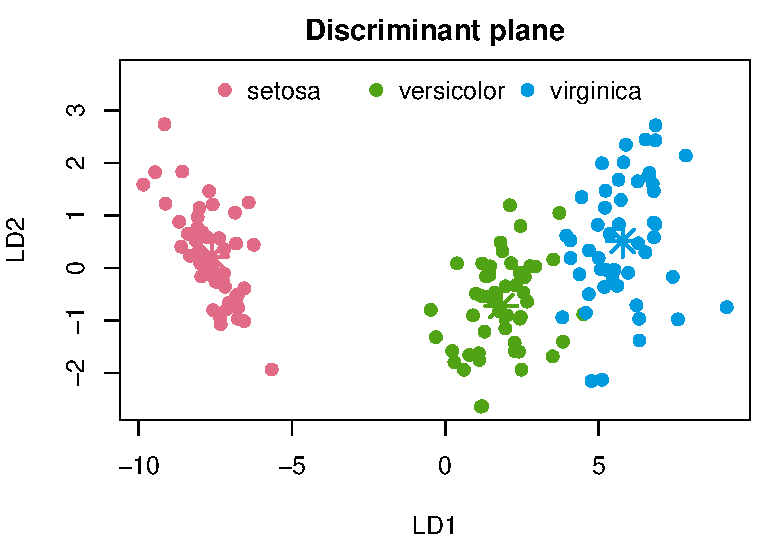
\includegraphics[width=0.6\textwidth]{figures/fig_plan.pdf}
\caption{Plan discriminant (\code{iris}) ; les \'etoiles sont les centro\"ides.}\label{fig:plan}
\end{figure}

%=====================================================================
\section{Application Shiny}
\code{ldaR6::run\_app()} lance une application \`a quatre \'etapes pens\'ee pour un d\'ebutant : (1)~\emph{Donn\'ees} : CSV/TSV (tabulation par d\'efaut), Excel ou exemples int\'egr\'es, aper\c{c}u et diagnostic des types ; (2)~\emph{Param\'etrage} : variable cible, variables explicatives et \emph{illustratives}, a priori, codage, s\'election, seuils, r\'etr\'ecissement, part d'apprentissage et graine, nombre de plis ; (3)~\emph{R\'esultats} : indicateurs cl\'es (pr\'ecisions d'apprentissage, de test et de validation crois\'ee, Wilks), fonctions de classement t\'el\'echargeables, tests, tableau color\'e du statut des variables et diagramme des contributions, matrices de confusion, plan discriminant avec individus de test, description des variables illustratives (corr\'elations, barycentres) et sortie \code{summary} compl\`ete ; (4)~\emph{Pr\'ediction} : formulaire g\'en\'er\'e dynamiquement avec les seules variables du mod\`ele (num\'erique ou liste de modalit\'es) et histogramme des probabilit\'es, ou \emph{pr\'ediction par fichier} (descripteurs seuls) avec export TSV des classes et des probabilit\'es. Les erreurs et avertissements du package deviennent des notifications lisibles. Les essais manuels dans RStudio confirment en local l'ajustement sur \code{iris} et \code{credit\_demo}, les sorties statistiques, la pr\'ediction individuelle et la pr\'ediction de trois individus depuis un CSV (\code{setosa}, \code{versicolor}, \code{virginica}). Aucun test automatis\'e \code{shiny::testServer} n'est revendiqu\'e dans cette livraison ; l'h\'ebergement en ligne n'est pas n\'ecessaire au sujet.

%=====================================================================
\section{Livrables, installation et limites}
\begin{itemize}
\item \textbf{GitHub} : code, aide, jeux de donn\'ees (\code{credit\_demo}, \code{iris}, fichier de nouveaux individus), tutoriel \code{TUTORIAL.md} (reproductible, en anglais), banc d'essai. D'ep\^ot pr\'evu sous \code{clark94/ldaR6} ; installation \emph{apr\`es publication} : \code{remotes::install\_github("clark94/ldaR6")}. Sa disponibilit\'e en ligne reste \`a v\'erifier avant remise.
\item \textbf{Plan B} : \code{ldaR6\_1.0.0.tar.gz} (\code{install.packages(..., repos=NULL, type="source")}).
\item \textbf{Qualit\'e} : \code{devtools::check(cran = FALSE)} ex\'ecut\'e localement sur R 4.4.2 : \textbf{0 erreur, 0 avertissement, 1 note} (\code{unable to verify current time}, contr\^ole des horodatages), dur\'ee 42,1 s. Aide au format Rd (\code{?LDA}) et tests \code{testthat} pr\'esents ; leur ex\'ecution s\'epar\'ee reste \`a confirmer.
\end{itemize}
\textbf{Limites.} (i) Hypoth\`eses gaussienne et d'homosc\'edasticit\'e (pas de QDA) ; (ii) la pseudo-inverse reste en $O(p^3)$ pour $p\gtrsim 2000$ ; (iii) pas de leave-one-out en forme ferm\'ee ni de parall\'elisation (la validation crois\'ee est s\'equentielle) ; (iv) $p$-values post-s\'election optimistes. \textbf{Perspectives} : DISQUAL pour les cat\'egorielles, ADL r\'egularis\'ee (lasso), parall\'elisation des plis, h\'ebergement de l'application.

%=====================================================================
\appendix
\section{Exemple de sortie de \code{\$summary()} (iris)}
\begin{small}
\begin{verbatim}
=== Linear Discriminant Analysis: summary ===
n = 150 | K = 3 | columns used = 4 | pooled df = 147

Classification functions (constant in first row)
                setosa versicolor  virginica
constant     -86.30847  -72.85261 -104.36832
Sepal.Length  23.54417   15.69821   12.44585
Sepal.Width   23.58787    7.07251    3.68528
Petal.Length -16.43064    5.21145   12.76654
Petal.Width  -17.39841    6.43423   21.07911

Global tests
     statistic   value     F df1 df2    p_value
 Wilks' lambda 0.02344 199.1   8 288 1.365e-112
Bartlett chi2 = 546.1 (df = 8), p < 2.2e-16

Canonical axes
 axis eigenvalue proportion canonical_corr   wilks   chi2 df    p_value
  LD1    32.1919   0.991213         0.9848 0.02344 546.12  8 8.871e-113
  LD2     0.2854   0.008787         0.4712 0.77797  36.53  3  5.786e-08

Confusion matrix (resubstitution)      Accuracy: 98.00%
            Predicted
Observed     setosa versicolor virginica
  setosa         50          0         0
  versicolor      0         48         2
  virginica       0          1        49
\end{verbatim}
\end{small}

\section{Utilisation minimale}
\begin{small}
\begin{verbatim}
library(ldaR6)
X <- iris[, 1:4]; y <- iris$Species
m <- LDA$new(selection = "none", encoding = "dummy")
m$fit(X, y)                             # apprentissage
m$summary()                              # sorties detaillees
m$predict(X[1:3, , drop=FALSE])          # trois classes
m$predict_proba(X[1:3, , drop=FALSE])    # probabilites
m$cross_validate(X, y, k = 5, seed = 1) # validation croisee
ldaR6::run_app()                         # application Shiny
\end{verbatim}
\end{small}

\section{Contenu de la suite de tests}
\code{test-lda-core.R} : \'equivalence avec \code{MASS::lda}, formule de classement, \code{manova}, lambda partiel, deux classes, API de pr\'ediction, validation des entr\'ees. \code{test-categorical-selection.R} : codages, modalit\'es inconnues, s\'elections forward/backward/both, \code{max\_vars}, pr\'ediction sur variables retenues, validation crois\'ee reproductible, variables illustratives. \code{test-robustness.R} : $p>n$, blocs de lignes, invariance d'\'echelle, classe singleton, lecture TSV, affichages et graphiques.


% Bibliographie finale placee sur une nouvelle page.
\clearpage
% Reference list retained in full and placed on the final page (physical page 12).
\phantomsection
\addcontentsline{toc}{section}{R\'ef\'erences}
\begin{thebibliography}{99}\small
\bibitem{sujet} Universit\'e Lumi\`ere Lyon~2, M2 SISE (2026--2027), \emph{Cr\'eation d'un package pour R : Analyse discriminante pr\'edictive, algorithmes et outils pour l'interpr\'etation des r\'esultats}, sujet de projet de Programmation R (support fourni par l'enseignant).
\bibitem{rako} R.~Rakotomalala (2020), \emph{Pratique de l'analyse discriminante lin\'eaire}, version~1.0, Universit\'e Lumi\`ere Lyon~2. Document PDF consultable : \url{https://eric.univ-lyon2.fr/ricco/cours/cours/Pratique_Analyse_Discriminante_Lineaire.pdf}.
\bibitem{wilks} S.~S. Wilks (1932), Certain generalizations in the analysis of variance, \emph{Biometrika} 24, 471--494. \url{https://doi.org/10.1093/biomet/24.3-4.471}
\bibitem{rao} C.~R. Rao (1973), \emph{Linear Statistical Inference and its Applications}, Wiley.
\bibitem{friedman} J.~H. Friedman (1989), Regularized discriminant analysis, \emph{JASA} 84(405), 165--175. \url{https://doi.org/10.1080/01621459.1989.10478752}
\bibitem{schafer} J.~Sch\"afer, K.~Strimmer (2005), A shrinkage approach to large-scale covariance matrix estimation, \emph{Stat. Appl. Genet. Mol. Biol.} 4(1). \url{https://doi.org/10.2202/1544-6115.1175}
\bibitem{saporta} G.~Saporta (2011), \emph{Probabilit\'es, analyse des donn\'ees et statistique}, Technip (DISQUAL).
\bibitem{esl} T.~Hastie, R.~Tibshirani, J.~Friedman, \emph{The Elements of Statistical Learning}, Springer. \url{https://hastie.su.domains/ElemStatLearn/}
\bibitem{mass} W.~N. Venables, B.~D. Ripley, \emph{Modern Applied Statistics with S} (package \code{MASS}). \url{https://cran.r-project.org/package=MASS}
\bibitem{sk} F.~Pedregosa et al. (2011), Scikit-learn : machine learning in Python, \emph{JMLR} 12, 2825--2830. \url{https://jmlr.org/papers/v12/pedregosa11a.html}
\bibitem{r6} W.~Chang, \emph{R6 : encapsulated classes with reference semantics}. \url{https://r6.r-lib.org/}
\bibitem{shiny} Posit, \emph{Shiny for R}. \url{https://shiny.posit.co/}
\end{thebibliography}

\end{document}
